%&latex
%
\providecommand{\main}{../..}
\documentclass[../../main.tex]{subfiles}

\begin{document}

%Main schema
% Population dynamics: what it is, why it is important
% - History: first models
% - Fisher Log Series and birth death processes
% - More data \Rightarrow Log-normal distribution. Its interpretation as a birth-death process leads to density dependence
% - Continuum limit (Kramers-Moyal expansion) \Rightarrow exact solution for time evolution \Rightarrow Fit of Species Turnover Distribution (STD)
% These models qualitatively explain the Relative Species Abundance (RSA) and also the Species Turnover Distribution (STD)
% To proceed further, we consider also the spatial distribution of species. The voter model (with speciation) is able to qualitatively explain both RSA and the beta diversity (and predicts scaling behaviours). A more precise beta diversity fit can be obtained by adding more parameters to the model - for example accounting for the Janzel-Connell effect. 


\lesson{31}{20/05/20}
Moreover, different species seem to interact \textit{weakly} with each other. Let's see how we can understand this from empirical data.

\medskip

Suppose we have $S$ species with population $n_1, \dots, n_S$. We consider the joint probability for a certain configuration $\bm{n}$, i.e. $\mathbb{P}(n_1, \dots, n_S)$. If the species are non-interacting, then the probability factorizes:
\begin{align*}
    \mathbb{P}(n_1, \dots, n_S) = p_1(n_1) p_2(n_2) \cdots p_S(n_S)
\end{align*}
And taking the $\ln$ of both sides would lead to:
\begin{align}\label{eqn:factor-p}
    \ln \mathbb{P}(n_1, n_2, \dots, n_S) = \sum_i \ln p_i(n_i)
\end{align}
However, if there is some kind of \textit{interaction} between different species, then (\ref{eqn:factor-p}) would contain other terms:
\begin{align*}
    \ln \mathbb{P}(n_1, n_2, \dots, n_S) = \sum_i \ln p_i(n_i) + \sum_{i < j} c_{i,j}(n_i, n_j) + \dots
\end{align*}

We can infer a specific form of $\mathbb{P}(n_1, \dots, n_S)$ just using the empirical information we have, without adding any other assumption, by using the MaxEnt principle. Let $S(\bm{P})$ be the information entropy of the joint distribution, defined as:
\begin{align*}
    S(\bm{P}) = - \sum_{\bm{n}} P(\bm{n}) \ln P(\bm{n})
\end{align*}
We choose the $P$ that maximizes $S(P)$ subject to certain observational constraints. For example, the average total population may be fixed:
\begin{align*}
    N = \langle \sum_i n_i \rangle = \sum_{\bm{n}} P(\bm{n}) \sum_i n_i
\end{align*}
If we use only this constraint, the MaxEnt distribution will be an exponential:
\begin{align*}
    P(\bm{n}) = K \exp(-\beta \sum_i n_i)
\end{align*}
which corresponds to the case of non-interacting species.

\medskip

To quantify interaction, we need to measure correlations between the populations of different species ($\beta$-diversity). For example, let's consider the Barro Colorado Island (BCI) forest. The dataset describes a region of size $\num{1000}\times\SI{500}{\m}$, recording the position and species of each tree. We can divide this area in $Q$ \textit{small} quadrants (let's say of size $\num{20}\times\SI{20}{\m}$). In each quadrant $a$, we measure the population $n_i^{(a)}$ of species $i$, and compute:
\begin{align}\label{eqn:maxent-bci}
    \langle n_i \rangle &= \frac{1}{Q} \sum_{j=1,\dots,Q} n_i^{(Q)}\\
    \langle n_i n_j \rangle &= \frac{1}{Q} \sum_{i=1,\dots,Q} n_i^{(Q)} n_j^{(Q)} \nonumber
\end{align}
To get useful results, it is convenient to consider only the most common species (e.g. the first $20$ \q{most frequent} ones), such that $n_i^{(Q)}$ are almost all far from $0$.

\begin{figure}[H]
    \centering
    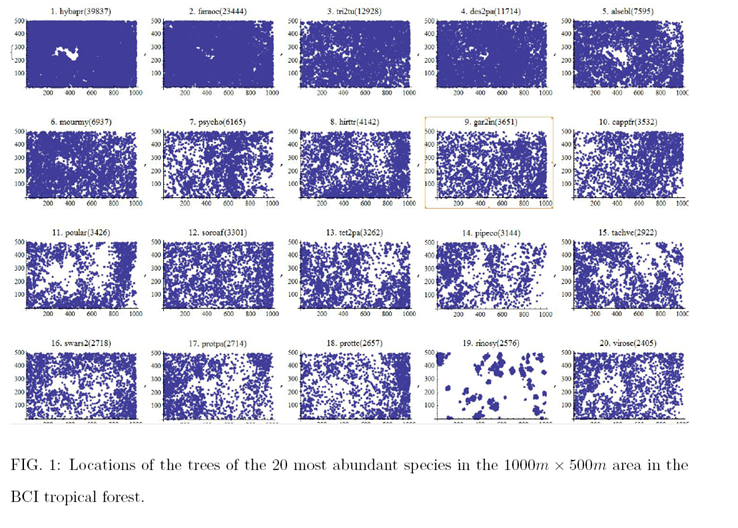
\includegraphics[width=0.8\textwidth]{\main/Images/tree-location.png}
    \caption{Location of trees of the $20$ most abundant species in the BCI dataset.}
    \label{fig:tree-location}
\end{figure}

Using (\ref{eqn:maxent-bci}) as constraints in a MaxEnt model, treating the $n_i$ as continuous variables for simplicity, the final distribution will be given by:
\begin{align*}
    \ln P(\bm{n}) &= K - \frac{1}{2} \sum_{i,j} (n_i - \langle n_i \rangle) M_{ij} (n_i - \langle n_i \rangle)\\
    M_{ij}^{-1} &= \langle n_i n_j \rangle - \langle n_i \rangle \langle n_j \rangle
\end{align*}
where $K$ is the normalization constant, and $\mathrm{M}$ acts as a correlation matrix. 

\medskip

If the species are non-interacting, then $\mathrm{M}$ is diagonal:
\begin{align*}
    \langle n_i n_j \rangle = \langle (n_i)^2 \rangle \delta_{ij}
\end{align*}

So, we can see how much interactions are important by examining the size of the non-diagonal elements of $\mathrm{M}$. The empirical results for the BCI forest are shown in fig. \ref{fig:bci-matrix}.

\begin{figure}[H]
    \centering
    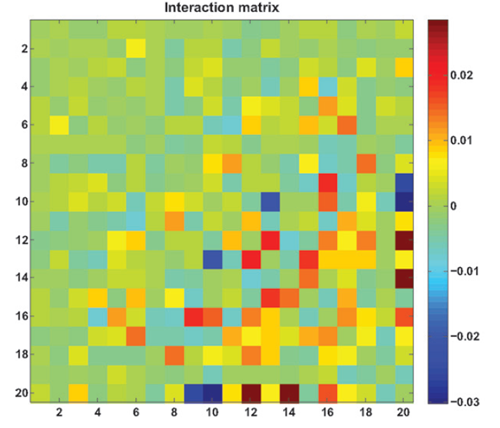
\includegraphics[width=0.8\textwidth]{\main/Images/bci-matrix.png}
    \caption{Correlation matrix for the top $20$ species in the BCI forest.}
    \label{fig:bci-matrix}
\end{figure}

The non-diagonal terms seem \textit{small} - but it is not exactly clear if it is right to say so, since we do not have any element to compare them to.

A trick is then to \textit{destroy} all correlations and examine the size of random fluctuations. To do this we can just \textit{relabel} each species inside each quadrant. In other words, inside each quadrant we permutate all \textit{species names} at random, and we repeat this (with different independent relabelling) for every quadrant. The result is a matrix with \textit{no real meaning}, which elements are the product of random chance (fig. \ref{fig:random-chance}).

\begin{figure}[H]
    \centering
    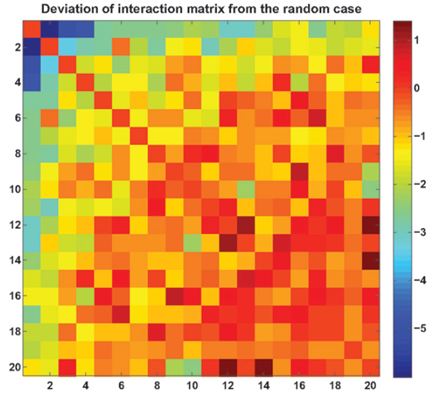
\includegraphics[width=.8\textwidth]{\main/Images/random-chance.png}
    \caption{Correlation matrix after random relabelling of all species in each quadrant.}
    \label{fig:random-chance}
\end{figure}

From this experiment we see that, if species were really distributed \textit{at random}, we would expect some relatively \textit{strong} interactions to arise from pure chance. This means that the matrix elements of fig. \ref{fig:bci-matrix} are indeed small, indicating that in nature, species that coexist \textit{do not interact much}. A possible explanation is that, for an ecosystem to be stable, the interactions between its parts must be either \textit{neutral} or \textit{cooperative} - otherwise several species would get extinct, destroying the equilibrium. However, the latter case is much more difficult to realize than the form, as it requires a more precise \q{order}, i.e. a lower information entropy. In nature, evolution optimizes species for survival through a series of random mutations. A system of weakly interacting individuals is more likely to arise from chance alone than a perfectly cooperative system, and still guarantees a low probability of extinction. 

\section{Models}
Following a semi-historical approach, we will now describe several models of population dynamics.
\begin{enumerate}
    \item \textbf{Birth-death processes} are one of the simplest way to \textbf{stochastically} model the growth and decline of populations. In section \ref{sec:birth-death}, we will see how including a Malthusian growth and a death rate proportional to population leads, at stationarity, to the \textbf{Fisher Log-Series}, one of the first function proposed to \textit{fit} empirical data. However, more modern datasets accounting also for rarer species lead to a population distribution that seems to follow a \textbf{log-normal function} - which can not be naturally produced by tweaking the parameters of a birth-death process. Fortunately, assuming birth/death rates that depend on the population itself (\textbf{density dependence}) can give similarly good results, while maintaining the overall model simple.
    
    \medskip

    In section \ref{sec:birth-death-continuum} we will then take the continuum limit of the birth-death process, obtaining a \textbf{deterministic} differential equation for the system's evolution. This can be used to predict the stationary distribution, and also to compute the Species Turnover Distribution (STD) - a sort of $\alpha$-diversity as a function of time. The latter is particularly useful to find the characteristic timescale of an ecosystem, i.e. the time needed for a population to recover from some sufficiently small external perturbation, such as human action. Alarmingly, that interval appears to be in the order of millennia in the case of Amazon rainforests.
    \item While birth-death processes are really useful to compute both $\alpha$-diversity and the STD, they miss entirely on the \textit{spatial} nature of ecosystems. The \textbf{voter model} is perhaps the most paradigmatic spatial model that is able to capture relevant features in the data. It is introduced in section \ref{sec:spatial-models}, where we state (just as an example) several key analytical results, and compare them with empirical evidence, with the aim of understanding the $\beta$-diversity of Amazon rainforests.
    
    \medskip

    Then, in section \ref{sec:voter-model} we show some full derivations in a simplified case, with the aim of understanding if, at equilibrium, several species will coexist (biodiversity), or only one will dominate (monodominance). As we will show, while the voter model can fit really well real data, it cannot explain how high biodiversity can be stable in nature - which is still one of the important unsolved problem in environmental statistical mechanics.
\end{enumerate} %TODO Add reference to contact model


\section{Birth-Death processes}\label{sec:birth-death}
We want now to construct a model based on the empirical observations we made regarding the distribution of species in forests. We make the following assumptions:
\begin{enumerate}
    \item Species in the same \textbf{trophic level} (number of steps from the start of the food chain) behave similarly.
    
    For example, \textbf{plants}  are all \textit{primary producers}, lying at trophic level $1$, and so we treat them all the same, without adding any specific details.
    \item Species interactions are taken into account only in the \textit{effective} \textbf{birth and death rates}. In other words, in this model different species interact only when a new organism is born, or dies.
    \item Different species are considered as \textit{independent} \textbf{realizations}  of the \textbf{same process}. For example, all species in a forest are like \q{different runs} of tossing the same coin - the ones that are most successfull are simply the \q{lucky} cases which have won many subsequent \textit{tosses}. They aren't, however, inherently different from the others - the coin that is tossed is always the \textit{same}, the game is fair.
    \item Species \textbf{behave} as if they are independent. Let $n_i$ be the population of the $i$-th species. The joint probability of all $S$ species having populations $n_1,\dots,n_S$ at time $t$ \textit{factorizes}:
    \begin{align*}
        \mathbb{P}(n_1, n_2, \dots, n_S; t) = \prod_{i=1}^S p_{n_i}(t)    
    \end{align*}   
    Note that, because of $3$, $p_{n_i}(t)$ depends only on the population $n_i$, and not on the particular species $i$. 
\end{enumerate}
At each timestep $\Delta t$ (which can be of order $\sim \SI{1}{y}$ for trees) a new individual is born with probability $b_n \Delta t$, or one existing organism dies with probability $d_n \Delta t$.

\begin{figure}[H]
    \centering
    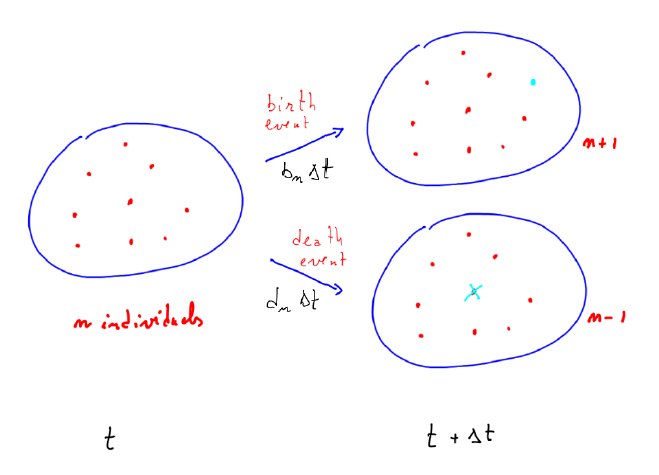
\includegraphics[width=0.8\textwidth]{\main/Images/birth-death-evo.png}
    \caption{} %TODO Add caption
    \label{fig:birth-death-evo}
\end{figure}

We can then write the Master Equation for a birth-death process as follows:
\begin{align}\label{eqn:birth-death-ME}
    \dot{\mathbb{P}}_{n} = \hlc{Yellow}{b_{n-1} \mathbb{P}_{n-1}(t)} + \hlc{SkyBlue}{d_{n+1}\mathbb{P}_{n+1}(t) }- (\hlc{SkyBlue}{b_n} +\hlc{Yellow}{ d_n}) \mathbb{P}_n(t) \qquad n\geq 0
\end{align}
The state with $n$ individuals \textit{gains probability} when one organism is born in the state with population $n-1$, or one dies from the state $n+1$. It instead \textit{loses probability} if either one individual is born or dies at the current state $n$. $b_n$ and $d_n$ are respectively the probabilities per unit time that a population of size $n$ increases/decreases by one unit. We take by convention $b_{-1} = 0$.

\medskip

Let $J_n$ be the \textit{net flux} of probability going from $n$ to $n+1$:
\begin{align}\label{eqn:p-flux}
    J_n \equiv b_n \mathbb{P}_n - d_{n+1} \mathbb{P}_{n+1}
\end{align} 
Then we can rewrite (\ref{eqn:birth-death-ME}) as a difference of fluxes:
\begin{align*}
    \dot{\mathbb{P}}_n = \hlc{Yellow}{J_{n-1}} - \hlc{SkyBlue}{J_n} \qquad d_0 \equiv 0; \> b_{-1} \equiv 0
\end{align*}
The \textbf{stationary state} is given by:
\begin{align*}
    \dot{\mathbb{P}}_n = 0 \quad \forall n\Leftrightarrow J_n = J_{n-1} = J_{n-2} = \dots = \text{Const.}
\end{align*} 
As $\sum_n \mathbb{P}_n = 1$, we expect $\mathbb{P}_n  \xrightarrow[n \to \infty]{} 0$, meaning that $J_n  \xrightarrow[n \to \infty]{} 0$. Thus the stationary state can be reached if:
\begin{align*}
    J_n = \dots = J_1 = 0
\end{align*}
And from (\ref{eqn:p-flux}):
\begin{align}\label{eqn:bd-db}
    0 \overset{!}{=} b_{n} \mathbb{P}_n - d_{n+1} \mathbb{P}_{n+1} \Big|_{\mathbb{P} = \mathbb{P}^{\mathrm{stat}}} \Rightarrow b_n \mathbb{P}_{n}^{\mathrm{stat}} = d_{n+1} \mathbb{P}_{n+1}^{\mathrm{stat}} \Leftrightarrow \frac{\mathbb{P}_{n+1}^{\mathrm{stat}}}{\mathbb{P}_n^{\mathrm{stat}}}  = \frac{b_n}{d_{n+1}} 
\end{align}
which is exactly the \textbf{detailed balance} condition. 

\medskip

Reiterating (\ref{eqn:bd-db}):
\begin{align}\label{eqn:p-stat}
    \mathbb{P}_{n}^{\mathrm{stat}} = \mathbb{P}_{n-1}^{\mathrm{stat}} \frac{b_{n-1}}{d_n} = \prod_{i=0}^{n-1} \frac{b_i}{d_{i+1}}   \mathbb{P}_0^{\mathrm{stat}}
\end{align}
However we expect that $b_0 = 0$, as no birth can occur in absence of individuals. So:
\begin{align*}
    \mathbb{P}_{n}^{\mathrm{stat}} = 0 \qquad n \geq 1
\end{align*}
or equivalently:
\begin{align*}
    \mathbb{P}_{n}^{\mathrm{stat}} = \delta_{n,0}
\end{align*}
So the only stationary state is the trivial one where there is no population.

\medskip

We say that the state $n=0$ is \textbf{absorbing}, as once reached cannot ever be left. Moreover, we know it will be reached for sure:
\begin{align*}
    \mathbb{P}_n(t)  \xrightarrow[t \to +\infty]{}  \delta_{n,0}
\end{align*}

It is then interesting to compute how much time on average is needed to reach it, i.e. the expected lifetime of every species before going extinct - this will be indeed the target of section \ref{sec:extintion-times}.

\medskip

For now, let's introduce a modification. Suppose the system is \textbf{open}. We know that species may \q{disappear} due to extinction or to migration, but we also expect species to \textit{arrive} from outside at a certain rate.
Then $b_0 > 0$ represents the probability \textit{per unit time} that a individual of a new species enters in the system. With this interpretation, $\mathbb{P}_n(t)$ is not anymore the probability that a given species has $n$ individuals, but rather the probability of observing a \q{random} species with $n$ individuals at time $t$ in the whole system. 

\medskip

Equation (\ref{eqn:p-stat}) holds also if $b_0 > 0$, but now $n=0$ is not anymore an absorbing state, nor the system's stationary state. 

Imposing normalization:
\begin{align*}
    1 \overset{!}{=} \sum_{n=0}^{+\infty} \mathbb{P}_n^{\mathrm{stat}} = \left[1+ \sum_{n=1}^{+\infty} \prod_{i=0}^{n-1} \frac{b_i}{d_{i+1}} \right] \mathbb{P}_0^{\mathrm{stat}}
\end{align*}
From this we can compute $\mathbb{P}_0^{\mathrm{stat}}$, and then use (\ref{eqn:p-stat}) to find every $\mathbb{P}_n^{\mathrm{stat}}$:
\begin{align*}
    \mathbb{P}_n^{\mathrm{stat}} = \begin{dcases}
        \frac{1}{1+ \sum_{k=1}^\infty \prod_{i=1}^{k-1} \frac{b_i}{d_{i+1}}} & n = 0\\
        \frac{\prod_{i=0}^{n-1} \frac{b_i}{d_{i+1}} }{1 + \sum_{k=1}^\infty \prod_{i=1}^{k-1} \frac{b_i}{d_{i+1}} }  & n \geq 1
    \end{dcases}
\end{align*}

Alternatively, we can neglect the species with $0$ population in the normalization:
\begin{align*}
    \sum_{n=1}^{+\infty} \mathbb{P}_{n}^{\mathrm{stat}} \overset{!}{=} 1
\end{align*}
This leads to the same expression for every $n$:
\begin{align}\label{eqn:p-stat2}
    \mathbb{P}_{n}^{\mathrm{stat}} = \frac{\displaystyle \prod_{i=0}^{n-1} \frac{b_i}{d_{i+1}}}{\displaystyle \sum_{k=1}^\infty \prod_{i=1}^{k-1} \frac{b_i}{d_{i+1}} }   
\end{align}

\subsection{Fisher Log Series}
Let's choose the birth-death rates as proportional to the population, except $b_0$ which is constant:
\begin{align*}
    b_n = \begin{cases}
        b_0 & n = 0\\
        n b & n \geq 1
    \end{cases} \qquad d_n = n\cdot d
\end{align*}
The proportionality constants $b$ and $d$ are respectively the per-capita birth/death rate.

\medskip

We can then compute the product at the numerator/denominator of (\ref{eqn:p-stat2}):
\begin{align*}
    \prod_{i=0}^{n-1} \frac{b_i}{d_{i+1}} &= \frac{b_0}{d} \prod_{i=1}^{n-1} \frac{ib}{(i+1)d} = \frac{b_0}{d} \left[\frac{b}{\cancel{2}d} \cdot \frac{\cancel{2}b}{\bcancel{3}d} \cdots \frac{\cancel{(n-1)}b}{nd}   \right] =\\
    &= \frac{b_0}{\cancel{d}} \textcolor{Red}{\frac{\cancel{d}}{b}}  \left(\frac{b}{d} \right)^{n-1} \frac{1}{n} \textcolor{Red}{\frac{b}{d}}  = \frac{b_0}{b} \left(\frac{b}{d} \right)^n \frac{1}{n} 
\end{align*}
This does not diverge, allowing to normalize the probability, if $b < d$:
\begin{align*}
    \sum_{n=1}^{+\infty} \frac{b_0}{d} \left(\frac{b}{d} \right)^n \frac{1}{n} = - \frac{b_0}{d} \ln \left(1-\frac{b}{d} \right)  \qquad b < d
\end{align*}
Substituting in (\ref{eqn:p-stat2}):
\begin{align}\label{eqn:fisher-log}
    \mathbb{P}_n^{\mathrm{stat}} = \frac{x^n/n}{|\ln(1-x)|} \qquad x \equiv \frac{b}{d} < 1 
\end{align}
which is known as the Fisher Log-Series. It was derived in the 1940s by Fisher, an ecologist studying the population of butterflies. Its original construction was however a bit strange, and filled with \textit{ad hoc} hypothesis. The link between the Fisher Log-Series and birth-death processes that we just showed is a much more recent development. 

\subsection{Data Binning and Preston Plots}
One problem when dealing with population data, is that $\mathbb{P}_n$ goes quickly to $0$ for $n \gg 1$, i.e. it is difficult to find samples with a high number of individuals all from the same species. This is because collecting a large sample requires huge efforts, and also because there are many species sharing the same environment.

\medskip

So, to better visualize population distributions, \textit{binning scheme} is required. One example is Preston's \textit{logarithmic} binning, were instead of plotting $\mathbb{P}_n$ directly, we plot $\tilde{\mathbb{P}}_i$ defined as follows:
\begin{align*}
    \tilde{\mathbb{P}}_i \equiv \sum_{n=2^i}^{2^{i+1}} \mathbb{P}_{n}^{\mathrm{stat}} \alpha_n \qquad \alpha_i = \begin{cases}
        \frac{1}{2} & \exists j \in \mathbb{N} \colon i = 2^j\\
        1 & \text{otherwise}
    \end{cases}
\end{align*}
Explicitly:
\begin{align*}
    \mathrm{Bin}(1) &= \mathbb{P}_{1}^{\mathrm{stat}} + \frac{1}{2} \mathbb{P}_2^{\mathrm{stat}} \\
    \mathrm{Bin}(2) &= \frac{1}{2} \mathbb{P}_2^{\mathrm{stat}} + \mathbb{P}_3^{\mathrm{stat}} + \frac{1}{2} \mathbb{P}_4^{\mathrm{stat}}  
\end{align*}

If $\mathbb{P}_n^{\mathrm{stat}}$ changes \textit{smoothly} (true if $n$ is sufficiently large), then we can approximate the $\mathbb{P}$ in an interval $[2^i, 2^{i+1}]$ with the value at the left side:
\begin{align*}
    \tilde{\mathbb{P}}_i \approx (2^{i+1} - 2^{i}) \mathbb{P}_{2^i}^{\mathrm{stat}} = 2^i \mathbb{P}_{2^i}^{\mathrm{stat}}
\end{align*}
So, approximately:
\begin{align}\label{eqn:Preston-approx}
    \tilde{\mathbb{P}}_n \approx n \mathbb{P}_n^{\mathrm{stat}}
\end{align}

Preston's binning is just a trick to approximately \textit{change variables} to a logarithmic scale. In fact, if we treat $n$ as a \textbf{continuous} variable (an approximation not bad if $n \gg 1$), and perform the change of random variables\footnote{Here we use $\ln$ instead of $\log_2$.} $z = \ln n$ we get:
\begin{align}\label{eqn:logscalebin}
    \tilde{\mathbb{P}}(z) \dd{z} = \mathbb{P}_n^{\mathrm{stat}}\dd{n} \Rightarrow \tilde{\mathbb{P}}(z) = \mathbb{P}_n^{\mathrm{stat}} \underbrace{\left|\dv{n}{z}\right|}_{n}  = \mathbb{P}_n^{\mathrm{stat}}n
\end{align}
which is exactly (\ref{eqn:Preston-approx}).

\medskip

For example, (\ref{eqn:logscalebin}) applied to (\ref{eqn:fisher-log}) leads to:
\begin{align*}
    \tilde{\mathbb{P}}(\ln n) = \frac{\cancel{n} \frac{x^n}{\cancel{n}}}{|\ln(1-x)|} = \frac{x^n}{|\ln(1-x)|} 
\end{align*}
which is just an exponential distribution.

\subsection{Log-Normal distribution}
While the data collected by Fisher agrees with his Log-Series model (fig. \ref{fig:fisher-log}), a new analysis with more data and using Preston's binning method clearly shows a deviation (fig. \ref{fig:preston-plot}).

\begin{figure}[H]
    \centering
    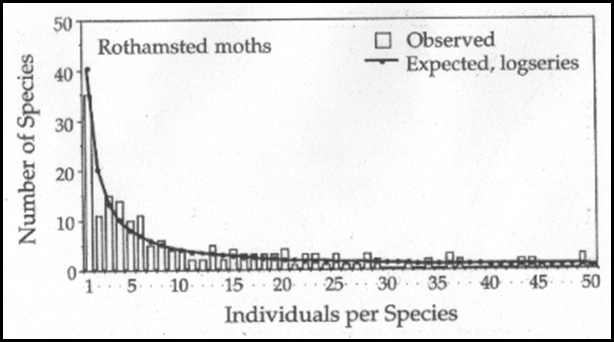
\includegraphics[width=0.6\textwidth]{\main/Images/fisher-log.png}
    \caption{Histogram of butterfly population sizes observed by Fisher, and compared with the Fisher Log-Series (\ref{eqn:fisher-log}).}
    \label{fig:fisher-log}
\end{figure}

\begin{figure}[H]
    \centering
    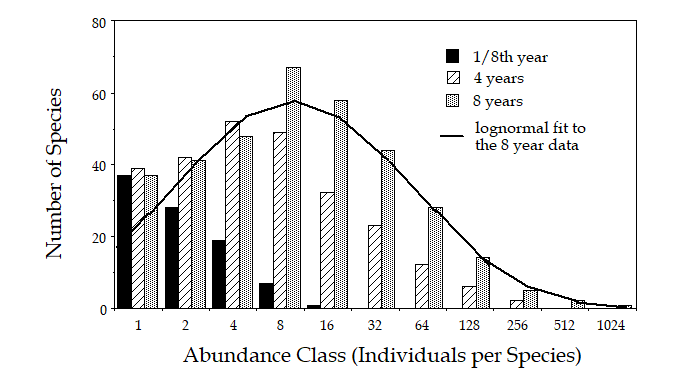
\includegraphics[width=0.8\textwidth]{\main/Images/preston-plot.png}
    \caption{Histogram (with Preston's logarithmic binning) of butterfly population sizes, comparing Fisher observations (darkest bars) with data collected over a much longer timespan. The black line corresponds to a log-normal fit.}
    \label{fig:preston-plot}
\end{figure}

Preston proposed a normal distribution for $\mathbb{P}_n$:
\begin{align*}
    \tilde{P}(i) \propto \exp\left(-\frac{(i-i_0)^2}{2 \sigma^2} \right)
\end{align*}
Since $i$ in a Preston's plot is just $\log_2 n$ - or $\ln n$ in our notation - this leads to a \textbf{log-normal distribution}:
\begin{align}\label{eqn:log-normal-dist}
    \tilde{P}(\ln n) = \frac{1}{\sqrt{2 \pi \sigma^2}}  \exp\left(-\frac{\left(\ln \frac{n}{n_0} \right)^2}{2 \sigma^2} \right)
\end{align}
which agrees with the newer and larger datasets (fig. \ref{fig:preston-plot}).

\medskip

To observe the full log-normal distribution, accurate measurements over a long period of time are required - while Fisher observed only the most frequent species, corresponding to a single \textit{tail} of the distribution (fig. \ref{fig:tail}).

\begin{figure}[H]
    \centering
    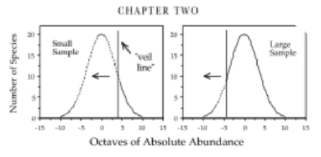
\includegraphics[width=0.6\textwidth]{\main/Images/tail.png}
    \caption{A small sample will contain only the most abundant species, corresponding to the \textit{rightmost} tail of the log-normal distribution. Everything else is hidden behind a \q{veil-line}, which can be \q{pushed further} only by increasing the sample size and the duration of the measurements.}
    \label{fig:tail}
\end{figure}

We now try to obtain a log-normal distribution as the stationary state of a birth-death process, by choosing accordingly $\{b_n\}$ and $\{d_n\}$:
\begin{align}\label{eqn:stat-log-normal}
    \mathbb{P}^{\mathrm{stat}}(n) \overset{!}{=} \frac{1}{n} \frac{1}{\sqrt{2 \pi \sigma^2}} \exp\left(-\frac{\left(\ln \frac{n}{n_0} \right)^2}{2 \sigma^2} \right) 
\end{align}
From (\ref{eqn:bd-db}) we must have:
\begin{align*}
    \frac{b_n}{d_{n+1}} &= \frac{\mathbb{P}^{\mathrm{stat}}(n+1)}{\mathbb{P}^{\mathrm{stat}}(n)} \underset{(\ref{eqn:stat-log-normal})}{=}  \frac{n}{n+1} \exp\left(-\frac{1}{2 \sigma^2} \left[\left(\ln \frac{\textcolor{Blue}{n+1}}{n_0} \right)^2 - \left(\ln \frac{\textcolor{Blue}{n}}{n_0} \right)^2\right]\right) =\\
    &\underset{\mathclap{n \gg 1}}{\approx}\>  \frac{n}{n+1} \exp\left(-\frac{1}{2 \sigma^2} \dv{n} \left[\ln \frac{n}{n_0} \right]^2 \right) = \frac{n}{n+1}\exp\left(-\frac{1}{2 \sigma^2} \frac{2}{n}\ln \frac{n}{n_0}   \right) =\\
    &= \frac{n}{n+1} \exp\left(-\frac{1}{2 n \sigma^2} \ln \frac{n}{n_0}  \right) 
\end{align*}
which is a quite \textit{strange} function - it is not easy to understand why a birth-death process should have this kind of parameters.

\medskip

%TODO Add introduction
An alternative is to assume that the per-capita birth and death rates have some dependence on the population itself (\textbf{density dependence}):
\begin{align}\label{eqn:density-dependence}
    \frac{b_n}{n} &= b + \frac{\tilde{b}}{n} + O\left(\frac{1}{n^2} \right)  \\ \nonumber
    \frac{d_n}{n} &= d + \frac{\tilde{d}}{n} + O\left(\frac{1}{n^2} \right)  
\end{align}
It is empirically known that \textit{small species} have a likelier chance of birth - for example because they interact \textit{less} with possible predators, and thus survive longer and have better chance for breeding.

\medskip

Let's assume that $\tilde{b}$ and $\tilde{d}$ are both proportional to (respectively) $b$ and $d$ with the same constant $c$:
\begin{align*}
    \tilde{b} = b c \qquad \tilde{d} = dc
\end{align*}
Then, neglecting higher order terms in (\ref{eqn:density-dependence}):
\begin{align*}
    b_n = b (n + c) \qquad \tilde{d} = d(n+c) \qquad n\geq 1
\end{align*}
and $b_0 > 0$ (we do not need to specify $d_0$). 

\medskip

We can then compute $\mathbb{P}_n^{\mathrm{stat}}$ (\ref{eqn:p-stat2}). First note that the ratio of $b_i$ to $d_{i+1}$ allows some simplification:
\begin{align*}
    \frac{b_i}{d_{i+1}} = \frac{b}{d} \frac{i+c}{i+1+c}  
\end{align*}
Thus: %TODO complete computations
\begin{align}\label{eqn:p-stat3}
    \mathbb{P}_n^{\mathrm{stat}} &= \mathbb{P}_0^{\mathrm{stat}} \prod_{i=0}^{n-1} \frac{b_i}{d_{i+1}}      = \underbrace{\mathbb{P}_0^{\mathrm{stat}} \frac{b_0}{d}}_{\equiv \alpha \cdot c}  \left(\frac{b}{d} \right)^n \frac{1}{n+c} = \alpha \left(\frac{b}{d} \right)^n \frac{c}{n+c} 
\end{align}
Imposing normalization:
\begin{align*}
    \sum_{n=1}^{+\infty} \mathbb{P}_n^{\mathrm{stat}} \overset{!}{=} 1 \Rightarrow \alpha^{-1} = \sum_{n=0}^\infty \left(\frac{b}{d} \right)^n \frac{c}{n+c} = F(1,c,c+1,b/d) \qquad b < d 
\end{align*}%TODO what happens if b > d?
where $F$ is the Gauss hypergeometric series %Abramowitz Stegun eq. 15.1.1 %TODO Add reference

Note that when $c \to 0^+$ we get back the Fisher Log-Series:
\begin{align*}
    \mathbb{P}_{n}^{\mathrm{stat}} = \frac{1}{n}\left(\frac{b}{d} \right)^n \frac{1}{-\ln (1-b/d)} 
\end{align*}

\begin{figure}[H]
    \centering
    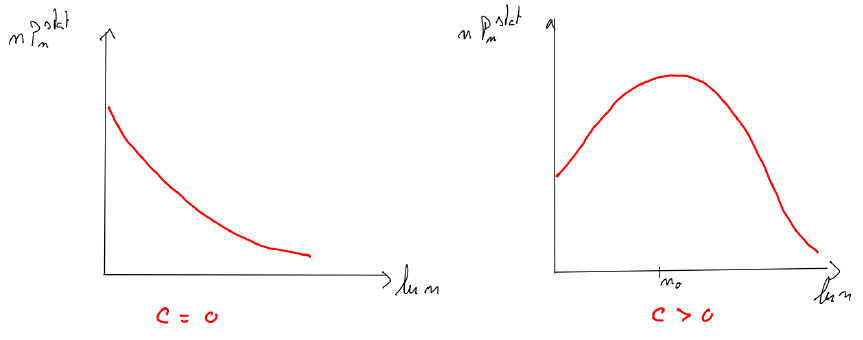
\includegraphics[width=0.9\textwidth]{\main/Images/preston-plots.png}
    \caption{Preston plots of (\ref{eqn:p-stat3}). For $c=0$ we obtain the Fisher Log-Series, while for $c > 0$ we get a log-normal distribution.}
    \label{fig:preston-plots}
\end{figure}

Empirically, $c=0$ is appropriate for very large sample sizes (e.g. forests at a continental scale), since the correction (\ref{eqn:density-dependence}) vanishes for $n \to +\infty$. For smaller sample sizes we use $c > 0$ instead (e.g. forests of $1 - 100 \si{hs}$).

$n_0$ may be determined as the maximum point:
\begin{align*}
    n_0 \colon \pdv{n} \ln \left(n \mathbb{P}_n^{\mathrm{stat} }\right) = 0 \Rightarrow n_0 \underset{(a)}{\approx}  \sqrt{\frac{c}{\ln b/d} } \approx \sqrt{\frac{c}{1-b/d} }
\end{align*}
The approximation in (a) is motivated by fits of real data, where $|b/d - 1| \lesssim 10^{-3}$ (tab. \ref{tab:fits}). Interestingly, this means that in real systems $b \approx d$, meaning that - in a sense - they are \q{near criticality}. 

When $b \approx d$, the average population size $\langle n \rangle$ diverges - as if taking the role of the correlation length in the critical Ising Model.  If $c=0$:
\begin{align*}
    \langle n \rangle &= \sum_{n=1}^{+\infty} n \mathbb{P}_n^{\mathrm{stat}} = \sum_{n=1}^{+\infty} n \left(\frac{b}{d} \right)^n \frac{1}{|\ln (1-b/d)|}  = \frac{b}{(d-b)|\ln(1-b/d)|} =\\
    &= \frac{b}{\delta |\ln \delta/d|}  \qquad \delta \equiv d-b > 0
\end{align*}
Note that $\langle n \rangle  \xrightarrow[\delta \to 0]{}  \infty$.

\begin{table}[htp]
    \centering
    \begin{tabular}{lcccccccc}
        \toprule \textbf{Plot}  & $S$ & $J$ & $\theta$ & $\alpha$ & $\beta$ & $x$ & $\chi^{2}$ & $p$ \\ \midrule
        Panama (BCI) & 225 & 21457 & 0.09642 & 2.8751 & 2.9745 & 0.99815 & 4.0935 & 0.9051 \\
        Yasuni, Ecuador & 821 & 17546 & 0.1857 & 6.1356 & 7.2429 & 0.99887 & 5.5337 & 0.7855 \\
        Pasoh, Malaysia & 678 & 26554 & 0.1581 & 1.4716 & 1.3855 & 0.99187 & 7.1739 & 0.4110 \\
        Korup, Cameroon & 300 & 24564 & 0.1381 & 4.0573 & 4.5751 & 0.99951 & 4.4298 & 0.9259 \\
        \bottomrule
    \end{tabular}
    \caption{Maximum likelihood estimates for parameters in the density dependent model (\ref{eqn:p-stat3}), with $b_n = (\alpha + n)b$, $d_n = (\beta + n)d$, $x = b/d$. $S$ is the number of species, $J$ the total population and $\theta$ is a biodiversity parameter. Note how $x \approx 1$ for all forests.}
\end{table}

The model (\ref{eqn:p-stat3}) seems to fit well real data (fig. \ref{fig:preston-fits2}). However, the simple form of density dependence for $b_n$ and $d_n$ in (\ref{eqn:density-dependence}) is not much realistic, as can be seen by comparing the theoretical prediction (\ref{fig:density-dependence}) with the actual data (\ref{fig:density-real}).


\begin{figure}[H]
    \centering
    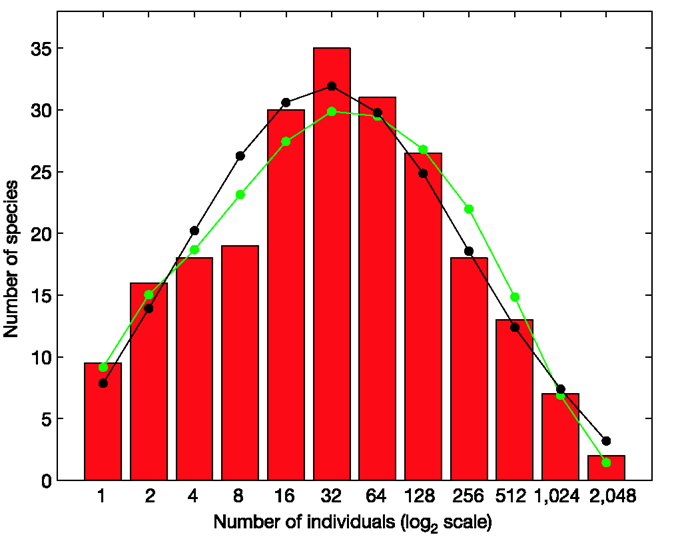
\includegraphics[width=0.8\textwidth]{\main/Images/preston-fits2.png}
    \caption{Preston plot of the Relative Species Abundance (RSA) of the BCI forest. The black line is a log-normal fit, while the green one is a fit with the density-dependent model (\ref{eqn:p-stat3}). Both curves fit the data really well, but (\ref{eqn:p-stat3}) comes from a well-defined model, not an \textit{ad-hoc} function.}
    \label{fig:preston-fits2}
\end{figure}



\begin{figure}[H]
    \centering
    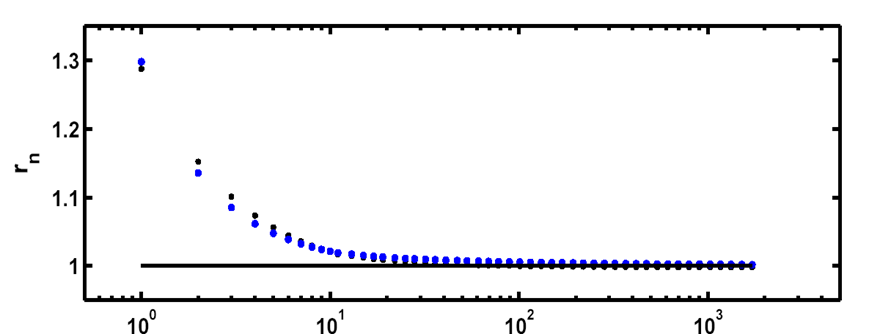
\includegraphics[width=0.8\textwidth]{\main/Images/density-dependence.png}
    \caption{Plot of $r_n = \frac{\mathbb{P}^{\mathrm{stat}}(n+1)}{\mathbb{P}^{\mathrm{stat}}(n)} \frac{n+1}{n} = x \frac{1+c/n}{1 + c/(n+1)}$. For $x = b/d \sim 1$, if $c = 0$ (Fisher Log-Series), then $r_n \equiv 1$ (black continuous line). Otherwise, if $c > 0$, $r_n$ depends on $n$, and is slightly $>1$ for small $n$ (blue and black points). Physically, this measures the \textit{survival advantage} of rare species (since they interact less with possible threats).}
    \label{fig:density-dependence}
\end{figure}

\begin{figure}[H]
    \centering
    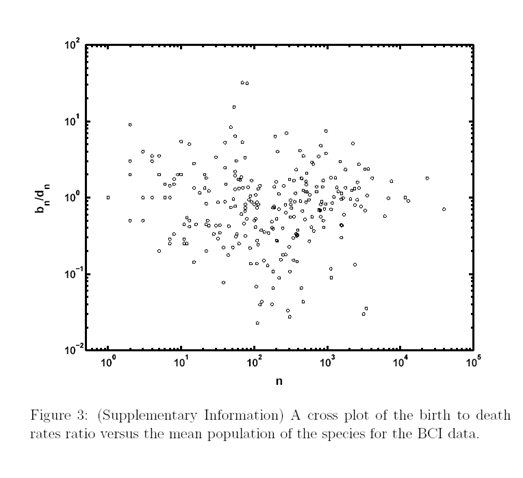
\includegraphics[width=0.7\textwidth]{\main/Images/density-real.png}
    \caption{Birth/death ratios for all species in the BCI forest. Note how $b_n/d_n$ does not tend to a constnat for $n \to \infty$, nor has any precise trend for $n$ small.}
    \label{fig:density-real}
\end{figure}


% \begin{figure}[H]
%     \centering
%     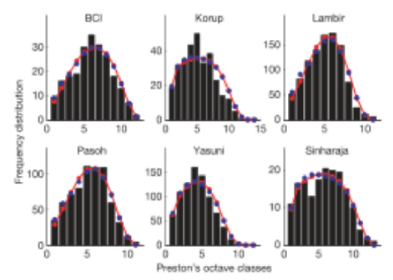
\includegraphics[width=0.8\textwidth]{\main/Images/preston-fits.png}
%     \caption{Example of fitting real data with the density-dependent model (\ref{eqn:p-stat3}).}
%     \label{fig:preston-fits}
% \end{figure}






\end{document}
